\documentclass{beamer}[10]
\usepackage{pgf}
\usepackage[danish]{babel}
\usepackage[utf8]{inputenc}
\usepackage{beamerthemesplit}
\usepackage{graphics,epsfig, subfigure}
\usepackage{url}
\usepackage{srcltx}
\usepackage{hyperref}
\usepackage{tikz}
\usepackage{moresize}
\usetikzlibrary{shapes.geometric, arrows}

\definecolor{kugreen}{RGB}{50,93,61}
\definecolor{kugreenlys}{RGB}{132,158,139}
\definecolor{kugreenlyslys}{RGB}{173,190,177}
\definecolor{kugreenlyslyslys}{RGB}{214,223,216}
\setbeamercovered{transparent}
\mode<presentation>
\usetheme[numbers,totalnumber,compress,sidebarshades]{PaloAlto}
\setbeamertemplate{footline}[frame number]

  \usecolortheme[named=kugreen]{structure}
  \useinnertheme{circles}
  \usefonttheme[onlymath]{serif}
  \setbeamercovered{transparent}
  \setbeamertemplate{blocks}[rounded][shadow=true]

\logo{\includegraphics[width=0.8cm]{KULogo}}
%\useoutertheme{infolines} 
\title{Image to text}
\author{Suraj Kiran S \\ Nakul A \\ Shinoj \\ Umesh U}
\institute{Government Engineering College, \\Sreekrishnapuram}
\date{} 



\begin{document}
\frame{\titlepage \vspace{-0.5cm}
}

\frame
{
\frametitle{Overview}
\tableofcontents%[pausesection]
}

\section{Literature survey}

\frame{
\frametitle{Literature survey}
Lorem ipsum dolor sit amet, consectetur adipiscing elit, sed do eiusmod tempor incididunt ut labore et dolore magna aliqua. Ut enim ad minim veniam, quis nostrud exercitation ullamco laboris nisi ut aliquip ex ea commodo consequat. Duis aute irure dolor in reprehenderit in voluptate velit esse cillum dolore eu fugiat nulla pariatur. Excepteur sint occaecat cupidatat non proident, sunt in culpa qui officia deserunt mollit anim id est laborum.
}
\section{Block diagram}

\frame{
\frametitle{Block diagram}
	\tikzstyle{box} = [rectangle, rounded corners, minimum width=3cm, minimum height=.5cm,text centered, draw=black, fill=red!30]
	\tikzstyle{square} = [rectangle, minimum width=3cm, minimum height=1cm, text centered, draw=black, fill=orange!30]
	\tikzstyle{arrow} = [thick,->,>=stealth]
	\begin{tikzpicture}[node distance=1.3cm]
	\node (1) [box] {Capture Image};
	\node (2) [box, right of=1,xshift=2cm] {Canny Transform};
	\node (3) [box, below of=2] {Skeletonization };
	\node (database) [square, right of=3,xshift=2.2cm,yshift=2.5cm] {Database };
	\node (4) [box, right of=3,xshift=2.2cm] {Machine Learning};
	\node (5) [box, below of=4] {Skeleton to text};
	\node (6) [box, below of=5] {Storage};
	\draw [arrow] (1) -- (2);
	\draw [arrow] (2) -- (3);
	\draw [arrow] (3) -- (4);
	\draw [arrow] (4) -- (5);
	\draw [arrow] (5) -- (6);
	\draw [arrow] (database) -- (4);
	
	\end{tikzpicture}
}
\section{Algorithm}

\frame{
\frametitle{Algorithm}
Lorem ipsum dolor sit amet, consectetur adipiscing elit, sed do eiusmod tempor incididunt ut labore et dolore magna aliqua. Ut enim ad minim veniam, quis nostrud exercitation ullamco laboris nisi ut aliquip ex ea commodo consequat. Duis aute irure dolor in reprehenderit in voluptate velit esse cillum dolore eu fugiat nulla pariatur. Excepteur sint occaecat cupidatat non proident, sunt in culpa qui officia deserunt mollit anim id est laborum.
}

\subsection{Canny Transform}

\frame{
\frametitle{Canny Transform/Edge Detection}
	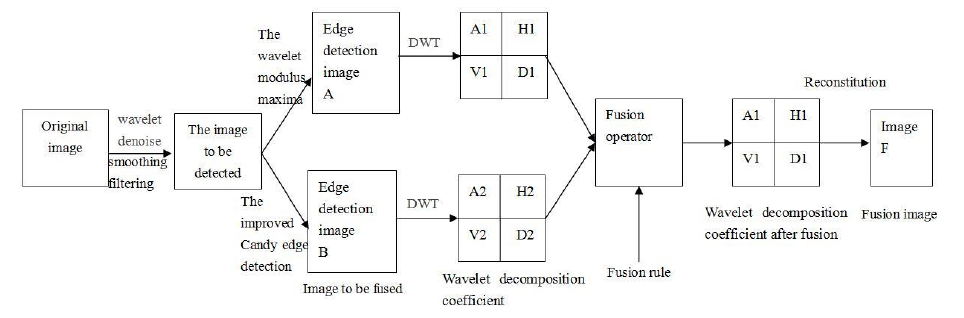
\includegraphics[scale=.3]{ct}
}

\subsection{Skeletonization}

\frame{
\frametitle{Skeletonization/Skinning}
jjjjjjjjj
	}
\begin{itemize}
\item First item
\item Second item
\item Third item
\end{itemize}

\subsection{Machine Learning}

\frame{
\frametitle{Machine Learning}
			\begin{itemize}
			\item \textbf{Decision tree learning}
				\newline
				\begin{itemize}
					\item \scriptsize Uses a decision tree as a predictive model.
					\item Predictive modeling uses statistics to predict outcomes.
				\end{itemize}
			\end{itemize}
			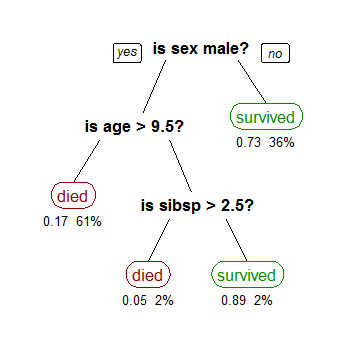
\includegraphics[scale=.4]{tree}
	}

\section{Execution}

\frame{
\frametitle{Implementation}
Lorem ipsum dolor sit amet, consectetur adipiscing elit, sed do eiusmod tempor incididunt ut labore et dolore magna aliqua. 
\begin{block}{Something important}
Einstein's formula
$$E=mc^2$$
\end{block}
}
\subsection{Intitial setup}

\frame{
\frametitle{Intitial setup}
\begin{itemize}
	\item Install Android Studio
	\item Install Anaconda library
	\item Create new project Android studio
	\item Download and import OpenCV library to Android studio project
	\end{itemize}
}

\subsection{Tools}

\frame{
\frametitle{Tools}
	\begin{itemize}
	\item Android Studio
	\item Anaconda
	\end{itemize}
}


\subsection{Dataset}

\frame{
\frametitle{Dataset}
	\begin{itemize}
	\item Skeleton of letters in the alphabet
	\item One to one maping of skeleton
	\end{itemize}
}


\section{Review report}

\frame{
\frametitle{Review report}
Lorem ipsum dolor sit amet, consectetur adipiscing elit, sed do eiusmod tempor incididunt ut labore et dolore magna aliqua. 
\begin{block}{Something important}
Einstein's formula
$$E=mc^2$$
\end{block}
}

\end{document}
